\section{Machbarkeitsstudie Stereokamera mit Raspberry Pi}
Vor der Anschaffung eines Kameramoduls für den Raspberry Pi, soll die Nutzbarkeit bewertet werden. Die Akzeptanzkriterien sind:
\begin{itemize}
    \item flüssige Ausgabe von Punktwolke (Avoidance benötigt $10-20$ \gls{fps})
    \item Erfassung großer Gegenstände, kleine Texturen können je nach Kamera und Lichtverhältnissen nicht erfasst werden
    \item Erfassung von Gegenständen im Nahbereich vor der Kamera, weitläufiger Hintergrund kann vernachlässigt werden
\end{itemize}

\acrshort{ros} stellt eine Beispiel-Videoaufnahme mit einer Auflösung von $640x480$ Pixeln und $15$ \gls{fps} Bildwiederholrate bereit, die von 2 Kameras als linke und rechte Perspektive aufgenommen wurde. Diese wird als Referenz für die Tests verwendet.

\subsection*{Durchführung}
\acrshort{ros} stellt die notwendige Software zur Verfügung. Mit dem Programm \textit{stereo\_image\_proc} können 2 Bilder (Linkes und Rechtes Bild) zu einem Tiefenbild zusammengeführt werden.

Die Software \acrshort{ros} kann als komplettes Packet von Docker\footnote{\url{https://hub.docker.com/_/ros/tags}} bezogen werden. Für den \gls{rpi} steht sie in der Version Noetic sowohl für \textit{arm32} als auch \textit{arm64v8} zur Verfügung, die Version wird entsprechend des Betriebssystems ausgewählt. Allerdings sind die Images zur allgemeinen Verwendung bestimmt. Somit enthält keines derer, kompilierte Software mit Optimierungen, die bspw. die Grafikbefehle des \gls{rpi} ausnutzen und so die Bildverarbeitung beschleunigen.

Optimierung steht im Kontext hier für eigene Kompilierung mit den C++-Compiler Flags \texttt{-march=native -O3}. Durch diese wird eine Anpassung auf den aktuell verwendeten Prozessor aktiviert. Speziell die Bildverarbeitung mittels OpenCV kann durch parallele Verarbeitung mit sog. Streaming-Befehlssätzen, ähnlich einer Grafikkarte, beschleunigt werden.

Um die Rechenkapazität des \gls{rpi} zu bewerten, wurden verschiedene Packete manuell kompiliert. Gleichzeitig wurden verschiedene Videoauflösungen zur Berechnung getestet. Verwendet wurde ein \gls{rpi} Model 4 B mit offiziellem 64-Bit Betriebssystem (Raspberry Pi OS). Der Quellcode zum Aufsetzen des Tests ist hinterlegt im GitHub\footnote{\url{https://github.com/aur20/T3000-autonomous_drone/tree/rpi_ros_bench_stereo}}. Das Vorgehen zum Durchführen der Tests ist beschrieben unter \footnote{\url{http://wiki.ros.org/stereo_image_proc/Tutorials/ChoosingGoodStereoParameters}}. Tabelle \ref{tab:bench_stereo_image_proc} zeigt die Ergebnisse in Bildrate je Einstellung und Auflösung.

\begin{table}[!ht]
    \caption{Benchmark zum Programm \textit{stereo\_image\_proc} auf dem \gls{rpi}}
    \begin{tabularx}{\textwidth}{>{\raggedright\arraybackslash}X|>{\raggedright\arraybackslash}X|>{\raggedright\arraybackslash}X}
    Versuch &   Auflösung normal (640x480)    &   Auflösung halbiert (320x240)\\
    \hline
    Standard Packete    &   6.3 &   14.7\\
    \hline
    Optimiertes OpenCV  &   6.9 &   14.7\\
    \hline
    Optimiertes OpenCV,\newline vision\_opencv und image\_pipeline & 6.7 & 14.6\\
    \label{tab:bench_stereo_image_proc}
    \end{tabularx}
\end{table}

\subsection*{Auswertung}
Selbst die Standardpackete erreichen gute Ergebnisse. Die internen Mechanismen beinhalten anscheinend bereits schon die meisten Optimierungen\footnote{siehe \enquote{Advanced SIMD}\url{https://en.wikipedia.org/wiki/AArch64}}. Zusätzlich wurden von den ursrpünglichen Entwicklern weitere Optimierungen im Zusammenhang mit \acrshort{ros} vorgenommen, die den Transfer von Bildinformationen verbessern.

Die Leistung des \gls{rpi} ist nicht ausreichend um hochauflösende Bilder
zu verarbeiten, aber dies wird auch für das Projekt nicht benötigt. Mit dem verwendeten Format wird das Maximum an Bildrate erreicht, es könnte also ein noch wenig besseres Format verwendet werden.

Der entstandene Aufwand steht in keinem Verhältnis zum Gewinn, in der finalen Anwendung können Standardpackete verwendet werden.

\section{Beschaffung Hardware Stereokamera}
Der \gls{rpi} 4 hätte hardware-technische Unterstützung mehrere Kameras anzuschließen. Allerdings besitzen die Modelle A und B nur immer einen notwendigen Header um ein Kameramodul anzuschließen.

Alternative Boards wurden von folgenden Projekten entwickelt:
\begin{itemize}
    \item Stereopi\footnote{\url{https://stereopi.com/}}
    \item Arducam\footnote{\url{https://www.arducam.com/product-category/stereo-vision-cameras/}}
\end{itemize}

Entscheidender Faktor bei der Beschaffung im Rahmen dieses Projektes ist der Preis, weshalb ein Stereopi gewählt wurde. Zusätzlich wird in jedem Fall ein leistungsstarker \gls{rpi} benötigt. Der aktuelle \textit{Stereopi v2} benötigt ein \textit{\gls{cm4}}, eine verkleinerte Version des \gls{rpi}, die als Aufsatz gedacht ist und selbst keine Anschlüsse besitzt. Beide Gerät sind in \ref{fig:stereopi_intro} abgebildet.

\begin{figure}[!ht]
    \centering
    \subfloat[][Raspberry Pi Compute Module 4 (\url{https://www.raspberrypi.com/products/compute-module-4/?variant=raspberry-pi-cm4001000})]{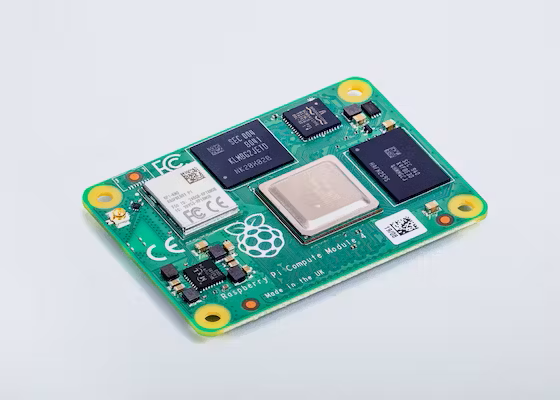
\includegraphics[width=0.4\textwidth]{images/cm4.png}}\hfill
    \subfloat[][Stereopi v2 (\url{https://wiki.stereopi.com/index.php?title=Main\_Page})]{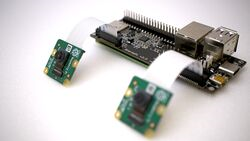
\includegraphics[width=0.4\textwidth]{images/stereopi.png}}\hfill
    \caption[Compute Module 4 und Stereopi]{Compute Module 4 und Stereopi}
    \label{fig:stereopi_intro}
\end{figure}

Da auf zur Zeit der Entwicklung keine \gls{cm4} auf dem Markt verfügbar sind, wird ein alternatives Board, welches Kompatibel zum \gls{rpi} sein soll, verwendet. Zum Einsatz kommt ein \textit{Radxa Compute Module 3}\footnote{https://wiki.radxa.com/Rock3/CM3}.

Zur Verbindung mit dem \textit{Stereopi v2} wurden 2 Kameras vom Typ \textit{Raspberry Pi Camera Module 2} besorgt. Diese bieten hochauflösende Bilder und Videos.

\subsection{Halterung für Platine und Kameras}
Um den \textit{Stereopi v2} und die Kameras zu verbinden, wurde eine Halterung entworfen und per 3D-Druck gefertigt. Die Modelle werden in Bild \ref{fig:stereopi_halterung} vorgestellt. Diese kann später an der Drohne montiert werden.

\begin{figure}[!ht]
    \centering
    \subfloat[][Hauptkörper für Stereopi-Platine mit RPI Compute Module]{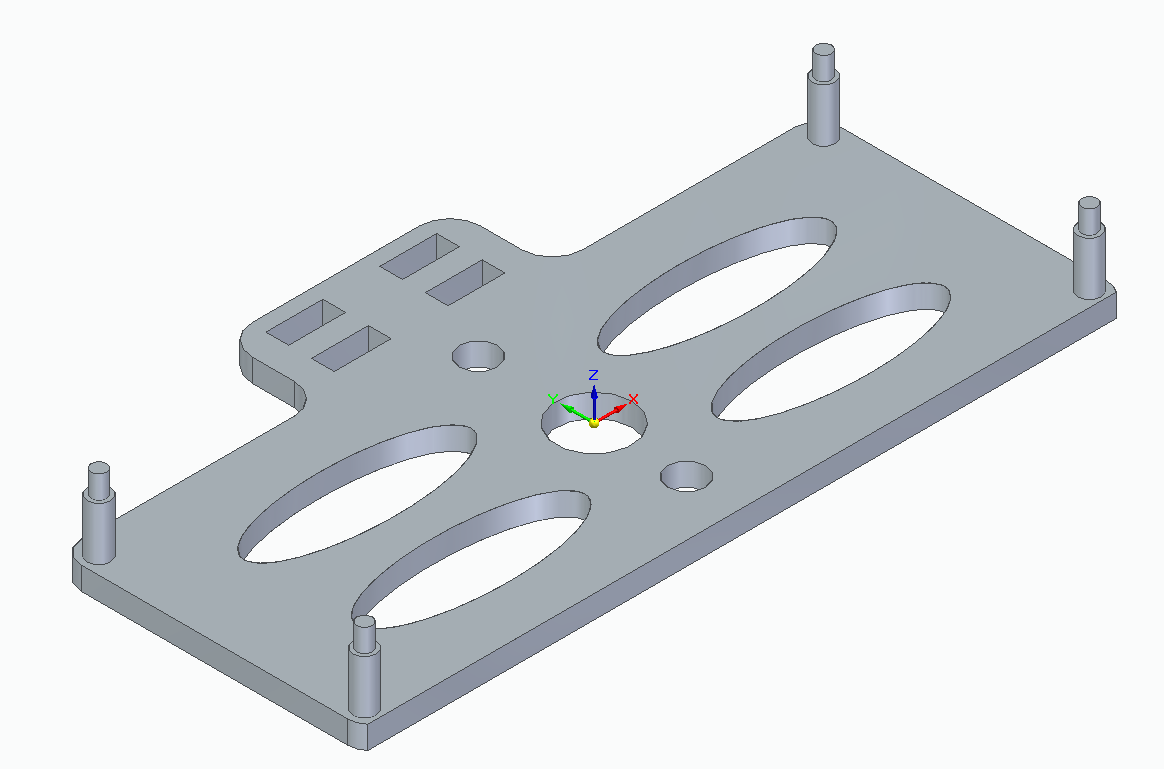
\includegraphics[width=0.4\textwidth]{images/stereopi_aufsatz_body.png}}\hfill
    \subfloat[][Steckaufsatz zur Halterung von 2 Kamera-Modulen]{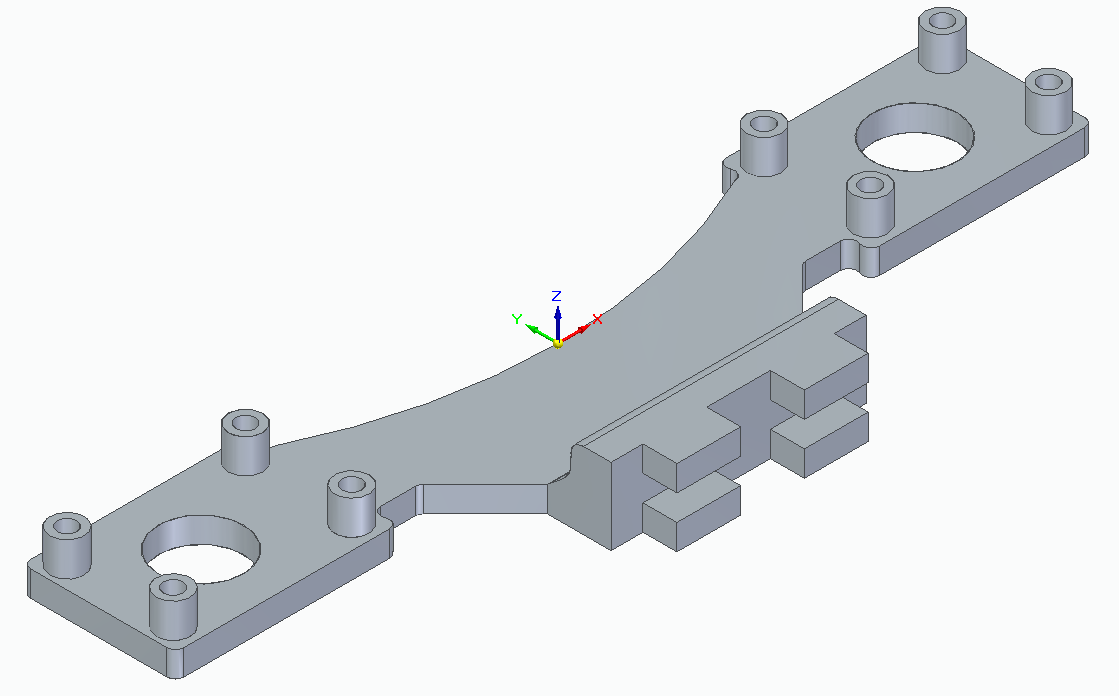
\includegraphics[width=0.4\textwidth]{images/stereopi_aufsatz_kam.png}}\hfill
    \caption[Halterung Platine Stereopi und 2 Kameras]{Halterung Platine Stereopi und 2 Kameras}
    \label{fig:stereopi_halterung}
\end{figure}

\subsection{Software auf dem Compute Module 4}
Das \gls{cm4} enthält einen verlöteten Flash-Chip mit $32GB$ Festspeicher. Das Betriebssystem kann mithilfe eines weiteren Computers geschrieben werden\footnote{siehe \url{https://wiki.radxa.com/Rock3/installusb-install-radxa-cm3-rpi-cm4-io}}. Weitere Schritte zur Einrichtung wurden als Script im Anhang unter \ref{listing:setup_stereopi.sh} hinterlegt. 

Um die Kameraanbindung des Stereopi zu aktivieren, ist eine speziell angepasste Software auf einem \gls{rpi} notwendig. Diese ist nicht mit dem Compute Module 3 von Radxa kompatibel.

Versuche im Rahmen dieser Arbeit haben gezeigt, dass das gesamte Linux Betriebssystem bereits einen veralteten Kernel verwendet. Es wurde zur Entwicklung minimaler Aufwand betrieben und kein weiterer Support bereitgestellt. Es kann offiziell noch zur letzten Version des 4er-Kernels geupdatet werden. Inoffiziell war es im Rahmen der Arbeit möglich auch den 5er-Kernel zu installieren, jedoch entfielen sämtliche Hardware-Funktionen (z.B. war \gls{wlan} nicht mehr verfügbar).

Für Anpassungen an Hardware-Funktionen muss bei Verwendung des 4er-Kernels die Datei \enquote{config.txt} in der Boot-Partition editiert, und anschließend das Script \enquote{update\_extlinux.sh} ausgeführt werden. Mit dem 5er-Kernel funktioniert dies nicht mehr, aber es gibt auch keine Dokumentation diesbezüglich.

Um die Kameraanbindung zu aktivieren, werden 2 Kanäle \gls{i2c} und 2 Kamerainterfaces benötigt. Diese sind in den Konfigurationsdateien des Compute Module 3 enthalten, müssen aber noch entsprechenden Pins zugewiesen werden.

Das Betriebssystem-Image von Radxa enthält weiterhin keinen (aktivierten) Grafiktreiber um etwaige Kameras auslesen zu können. Entweder muss das offizielle CM3-IO Board verwendet werden (welches auch mehrere Kameraanschlüsse besitzt) oder diese tauchen nach Erkennen einer Kamera automatisch auf.\newline

Im Rahmen dieser Arbeit war es nicht möglich die Kameras zu verwenden, zum Einsatz kommen nur die Ultraschallsensoren.

\section{Einrichtung der Ultraschallsensoren}
In diesem Kapitel wird die Verwendung der Ultraschallsensoren in Verbindung mit \acrshort{ros} beschrieben.

\subsection{Erzeugen einer Punktwolke}
Ein Beispiel zur Erzeugung von Punktwolken mit Python ist gegeben unter \footnote{\url{https://docs.ros.org/en/noetic/api/rospy_tutorials/html/publish__pointcloud2_8py_source.html}}, es erzeugt das Bild \ref{fig:ultra_pc_ex}. (Dieses bewegt sich gleichzeitig noch wellenartig.)

Das \acrshort{ros}-Punktwolkenformat definiert eine Klasse mit den Eigenschaften:
\begin{description}
    \item[Header:]
    \begin{itemize}
        \item[]
        \item[$\cdot$] stamp - aktueller Zeitstempel
        \item[$\cdot$] frame\_id - Kennzeichnung zur Transformation
    \end{itemize}
    \item[Fields:] Liste von Eigenschaften der Punkte, beihaltet x-,y-,z-Position sowie Farbattribute
    \item[Points:] Liste von Punkten, jeder Punkt im Format wie \enquote{Fields}
\end{description}

Der Zeitstempel wird mit jeder publizierten Nachricht auf die aktuelle Zeit angepasst.

Für die Anwendung im Projekt ist muss die \enquote{frame\_id} eine entsprechende Transformation von der lokalen Position der Drohne besitzen. Im einfachsten Fall wird die Drohne selbst als Ursprungspunkt des Bildes angenommen sodass keine Transformation benötigt wird. Somit entspricht die verwendete \enquote{frame\_id} vorerst immer \enquote{fcu}.

Als Fields kommen die 3 Raumkoordinaten und ein Farbfeld (Achtung hier Abweichung vom Beispiel) zum Einsatz. Das Farbfeld dient der Darstellung in \textit{rviz}, spielt aber für den Einsatzzweck keine Rolle.\\

Zur Erprobung wird eine Liste von Punkten angelegt. Diese befinden sich in 4 Ecken um den Koordinatenursprung (\enquote{fcu}) und einmal direkt darüber. Die Abstände sind jeweils $1m$ in x- und y-Richtung sowie $1m$ in z-Richtung für den z-Punkt. Die Topic der Nachricht wird mit $4Hz$ veröffentlicht, was der Update Rate der Sensoren entspricht \cite[Kapitel 4.4]{markusreinErweiterungBestehenderDrohnen2023}. Das Script ist im Anhang \ref{listing:pcl_test.py} abgedruckt, das Ergebnis zu sehen hier in Bild \ref{fig:ultra_pc_test}. Zur Zeichnung im Bild gibt es noch keine Transformation. Das Koordinatensystem \enquote{fcu} wird daher als Ursprung angenommen (die Einstellung ist oben links in \textit{rviz} zu sehen).

\begin{figure}[!h]
    \centering
    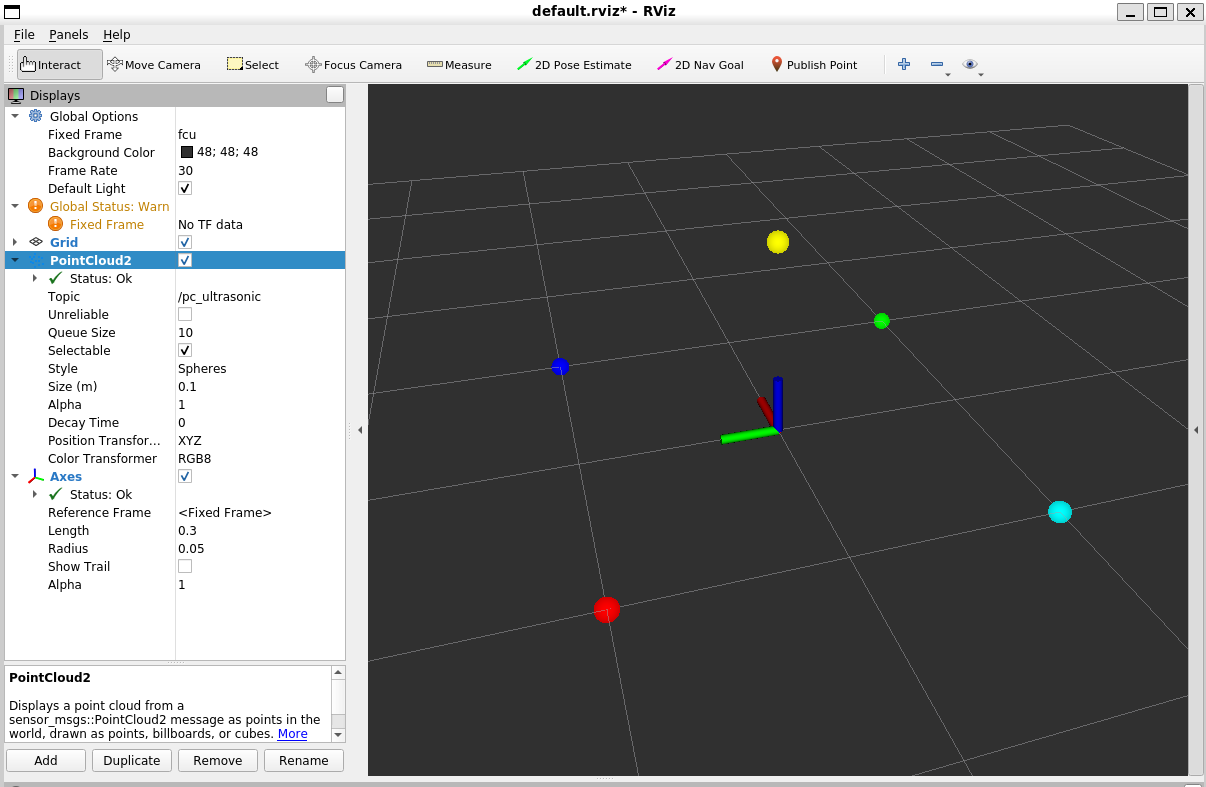
\includegraphics[width=0.7\linewidth]{images/ultra_pc_test.png}
    \caption[Erprobung von Punktwolkenformat]{Erprobung von Punktwolkenformat in \textit{rviz}: die Punkte jeweils im Abstand von $1m$ zum Ursprung. Als Referenz wurde noch ein Koordinatensystem am Ursprung eingezeichnet, bei diesem enspricht rot der x-Achse=rot, grün der y-Achse, blau der z-Achse}
    \label{fig:ultra_pc_test}
\end{figure}

Zur weiteren Erprobung wird die Simulation gestartet. Die 5 erzeugten Punkte sollten sich gemeinsam mit der Drohne bewegen. In Bild \ref{fig:ultra_pc_test_sim} wurde die Software-Simulation mit Stereokamera gestartet. Anschließend wurde das Script zur Erzeugung von Punktwolken gestartet und in \textit{rviz} hinzugefügt. Zu sehen ist die \enquote{Drohne} (Ursprung der Drohne) mit Punkten, welche sich mitbewegen. Die Bewegung der Punkte ist durch die geringe Update Rate immer etwas später als die der Drohne. Dies sollte aber kein Problem sein, denn es spiegelt das reale Verhalten (die Punkte bleiben stehen aber die Drohne bewegt sich auf diese zu/weg) wieder.

\begin{figure}[!h]
    \centering
    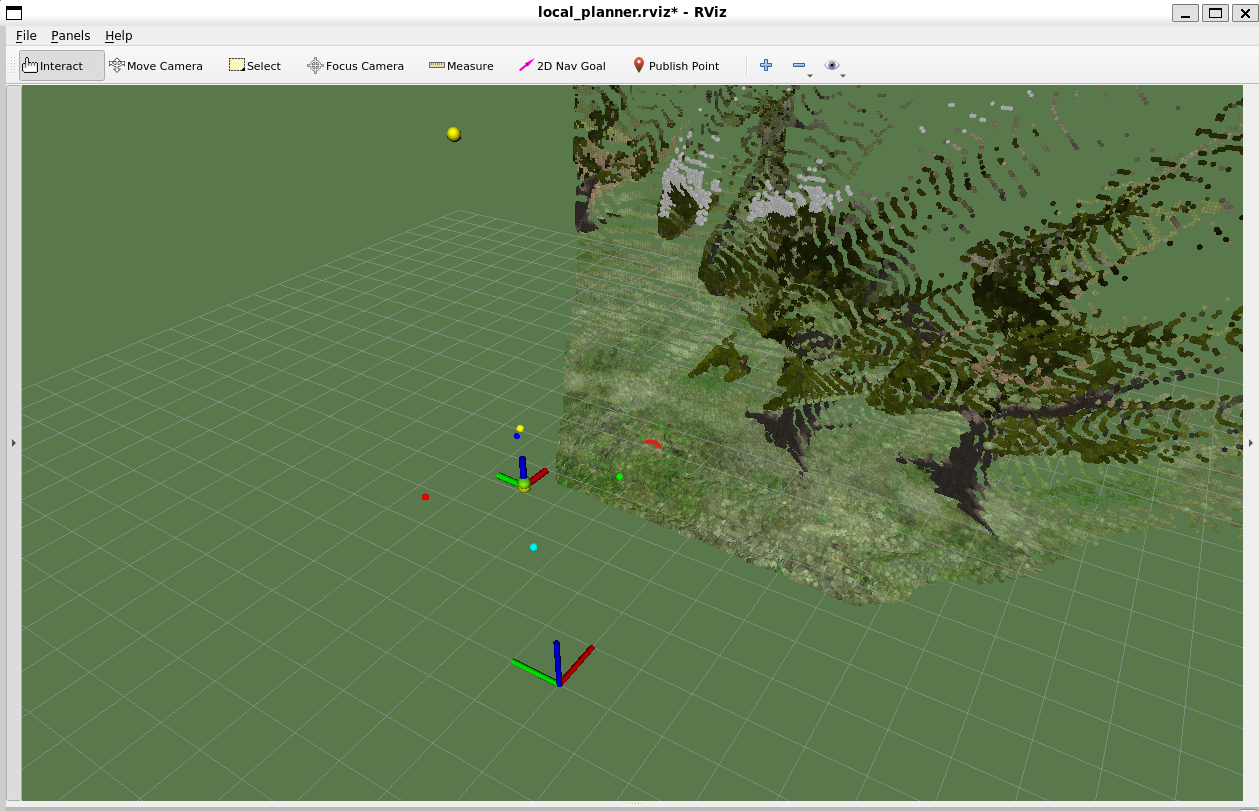
\includegraphics[width=0.7\linewidth]{images/ultra_pc_test_sim.png}
    \caption[Erprobung von Punktwolkenformat mit Simulator]{Erprobung von Punktwolkenformat mit Simulator: die Drohne befindet sich in der Luft vor den Bäumen, um sie herum sind die erzeugten Punkte eingezeichnet}
    \label{fig:ultra_pc_test_sim}
\end{figure}

\subsection{Software der Sensoren}\label{chap:arduino_sensors}
Der Algorithmus zum Auslesen der Sensoren wurde bereits für \cite[Kapitel 4.4]{markusreinErweiterungBestehenderDrohnen2023} entworfen, aber die Anwendung noch nicht dokumentiert. Der Code des Projektteils ist auf GitHub unter \footnote{\url{https://github.com/aur20/T3000-autonomous_drone/tree/arduino_sensors}} hinterlegt. Er besteht aus 2 Teilen:

Die \textbf{\large Arduino Firmware} liest die Sensoren aus und stellt Daten per \gls{i2c} zur Verfügung.

Das Auslesen der Sensoren ist mit der notwendigen Verzögerung verbunden, um eventuellen Echos von Ultraschall vorzubeugen. In \ref{listing:ultra_arduino_loop} dargestellt ist ein Ausschnitt aus der loop()-Schleife, die fortwährend immer durchlaufen wird. Der gezeigte Code kommt 4-mal vor, jeweils mit geänderten Pins der Sensoren (Zeile 187) und geänderten Indizes (Zeile 188-190). In der ersten gezeigten Zeile wird der jeweilige Sensor ausgelesen. Dazu wird mittels einer Arduino-internen Funktionen bis zum empfangenen Echo gewartet und die Zeit zurückgegeben. Anschließend wird der gefilterte Sensorwert berechnet. Der ungefilterte und gefilterte Wert werden jeweils in ein Array eingetragen. Zuletzt erfolgt das Warten, mit einer groben Annäherung: das Makro $PAUSE\_MEAS$ steht für $60ms$. Davon abgezogen wird die Zeit, die bereits auf das Echo gewartet wurde in Millisekunden. Arduino selbst stellt eine Verzögerungsfunktion in Mikrosekunden bereit, dieses sollte jedoch nicht für Verzögerungen länger als \enquote{a few thousend microseconds}\footnote{\url{https://www.arduino.cc/reference/en/language/functions/time/delaymicroseconds/}} verwendet werden, und funktioniert auch nur bis zu $16ms$ Verzögerung. Um die Zeit von Mikrosekunden in Millisekunden umzurechnen, muss durch $1000$ geteilt werden. Im Programm wird stattdessen $10$ mal nach rechts geschoben, was einer Division durch $1024$ entspricht. Die Verarbeitung von Schiebeoperationen ist wesentlich schneller als eine Division. Letztere kann im benötigten Zahlenbereich von kleiner $30.000$ zwar mit Integer Variablen umgesetzt werden, benötigt dann aber nach \footnote{\url{https://forum.arduino.cc/t/speed-of-math-operations-particularly-division-on-arduino/90726/5}} immer noch bis zu $15ms$, was die Messfrequenz beeinflussen würde. Außerdem hat der Prozessor bereits Zeit mit der Berechnung des Filters verbracht, sodass die Wartezeit lediglich eine Annäherung an $60ms$ ist, für das Ergebnis spielt dies keine Rolle.  

\begin{listing}[!ht]
    \cccode[firstline=187, lastline=191]{snippets/ultrasonic_arduino.ino}
    \caption{Ausschnitt der Arduino Firmware: loop()-Schleife}
    \label{listing:ultra_arduino_loop}
\end{listing}

Neben dem Auslesen der Sensoren stellt sich der Arduino als \gls{i2c}-Slave zur Verfügung. Er reagiert auf einzelne zugesendete Buchstaben und Zahlen und sendet eine entsprechende Antwort. Derzeit implementiert sind die Funktionen wie in \ref{tab:ultra_arduino_impl_i2c} aufgezeigt.

\begin{table}[!ht]
    \centering
    \caption{Verfügbare Kommandos zum Auslesen der Sensordaten auf Arduino}
    \begin{tabularx}{0.7\textwidth}{ l | l }
    Kommando & Anwort \\ \hline
    eine der Zahlen $1$-$4$ & jeweiliger Sensorwert, gefiltert\\
    Buchstabe \enquote{a} & alle Sensorwerte, gefiltert\\
    Buchstabe \enquote{r} & alle Sensorwerte, ungefiltert
    \label{tab:ultra_arduino_impl_i2c}
    \end{tabularx}
\end{table}

Das \textbf{\large Python Script} auf dem \gls{rpi} gibt Messwerte aus oder speichert diese als \acrshort{csv}-Datei ab.

Derzeit stehen die Scripte \textit{ultrasonic\_i2c\_reader.py} und \textit{ultrasonic\_i2c\_csvwriter.py} zur Verfügung. Sie verhalten sich nahezu gleich. Bei ersterem kann durch die Eingabe eines Zeichens ein bestimmter Wert an den Arduino gesendet werden. Die Antwort wird entsprechend auf der Konsole ausgegeben.\\
Beim zweiten Script kommt nur der Buchstabe \enquote{a} zum Einsatz. Es wird die Antwort geparst und mit aktuellem Zeitstempel in die Datei eingetragen. \ref{listing:ultra_rpi_impl_i2c} zeigt einen Ausschnitt aus der Schleife des zweiten Scriptes. In Zeile 25 werden die Daten per \gls{i2c}-Verbindung gelesen. Um die 16 Byte Binärdaten als Fließkommazahlen zu interpretieren wird das Packet \enquote{struct} verwendet. Im Beispiel werden die Daten in Zeile 28 als Fließkommazahlen im Little-Endian Format interpretiert. Die Funktion \textit{struct.iter\_unpack} liefert anschließend ein iterierbares Objekt (\enquote{Each iteration yields a tuple as specified by the format string.}\footnote{\url{https://docs.python.org/3/library/struct.html}}). Um den Inhalt zu extrahieren wird eine Lambda-Funktion innerhalb der Funktion \textit{map} verwendet, dies hat zur Folge dass jedes Tupel einzeln betrachtet werden kann. Es wird die jeweilige Zahl extrahiert und in einer Liste angelegt. Die Liste wird zusammen mit der derzeitigen Zeit jeweils ausgegeben und in die Datei geschrieben.

\begin{listing}[!ht]
    \pycode[firstline=25, lastline=30]{snippets/ultrasonic_i2c_csvwriter.py}
    \caption{Ausschnitt des Python Scriptes zum Auslesen der Sensordaten}
    \label{listing:ultra_rpi_impl_i2c}
\end{listing}

\subsection{Einbinden der Sensoren}
Als nächster Schritt wurden die vorliegenden Programme miteinander vereinigt.
Vom letzten Script werden jeweils alle 4 Sensoren ausgelesen. Aufgrund der Ungenauigkeit der Messwerte, wurde der Wertebereich nochmals eingeschränkt und beträgt hier $3m$. Größere Werte (beinhaltet Werte außerhalb der Reichweite, die mit $4m$ gesendet werden) werden schlichtweg ignoriert. Die Angaben für die Punktwolke werden auf Meter umgerechnet.

Das Projekt liegt separat auf GitHub\footnote{\url{https://github.com/aur20/T3000-autonomous_drone/tree/rpi_ros_ultrasonic}} und kann innerhalb zukünftiger Container direkt eingebunden werden.
